\chapter{Coherence walls and the coherence optimum}\label{ch:walls}
% Numbers: docs/book/figscripts/fig_p3_devices_g3.py (a/b = 3.45 for 0.65).

\section{Three components of a gate error}

The qubit gauge (Section~\ref{sec:devicegauges}) splits a superconducting two-qubit error into three parts:
\begin{equation}
 p_{2Q}=p_{\mathrm{coh}}+p_{\mathrm{mat}}+p_{\mathrm{ctrl}} .
 \label{eq:pdecomp}
\end{equation}
Here $p_{\mathrm{coh}}$ is the error from finite $T_1$ and $T_2$ over the gate time. For a gate of duration $t_g$,
$p_{\mathrm{coh}}\approx t_g/T_1+t_g/T_\phi$ up to state-averaging factors~\cite{Abad2022} \derived. The second term,
$p_{\mathrm{mat}}$, is the error contributed by the two-level-system (TLS) population of the device's surfaces and
interfaces. The gauge takes it to grow as $T_1$ approaches the ceiling $T_{1,\mathrm{free}}$ that this population allows.
The third, $p_{\mathrm{ctrl}}$, is the control and crosstalk overhead. Only the first term follows from standard theory.
The split between the second and the third is a model \conjecture.

\section{A coherence optimum}

The simplest forms with these properties are $p_{\mathrm{coh}}=a/T_1$ and $p_{\mathrm{mat}}=b/(T_{1,\mathrm{free}}-T_1)$,
with $a$ and $b$ constants of the device. Their sum is smallest where $a/T_1^2=b/(T_{1,\mathrm{free}}-T_1)^2$, that is at
\begin{equation}
 \frac{T_1^*}{T_{1,\mathrm{free}}}=\frac{r}{1+r},\qquad r=\sqrt{a/b}.
 \label{eq:t1star}
\end{equation}
\derived\ (within the model). Beyond $T_1^*$ a device on the same material that gains $T_1$ loses more to the material
term than it gains in coherence. The value $T_1^*=0.65\,T_{1,\mathrm{free}}$ used by the qubit gauge corresponds to
$a/b=(0.65/0.35)^2=3.45$ \calc. It is therefore a property of the device constants, not a universal number
(Figure~\ref{fig:coherence_optimum}). The model itself is a \conjecture: no physical mechanism has been identified by
which a rising $T_1$ would raise $p_{\mathrm{mat}}$. In standard theory TLS loss lowers $T_1$~\cite{Martinis2005,Muller2019};
the material term can rise while $T_1$ rises only if a second channel, such as crosstalk through a denser coupler
graph, changes at the same time.

\begin{figure}[htbp]\centering
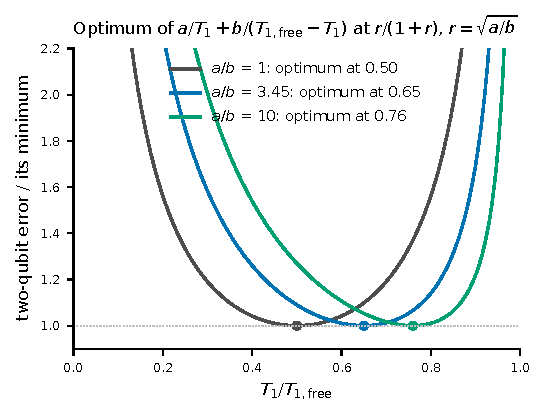
\includegraphics[width=0.62\textwidth]{figures/part3/fig_p3_coherence_optimum.pdf}
\caption{The model $p=a/T_1+b/(T_{1,\rm free}-T_1)$, each curve divided by its own minimum, for $a/b=1$, 3.45 and 10.
The optimum sits at $T_1^*/T_{1,\rm free}=r/(1+r)$ with $r=\sqrt{a/b}$; the value 0.65 needs $a/b=3.45$.
\derived\ (form) \calc\ (values)}\label{fig:coherence_optimum}
\end{figure}

\section{Where the ceiling comes from}

Most TLS loss in present transmons sits in the amorphous oxides at the metal--air, metal--substrate and substrate--air
interfaces and on the junction leads~\cite{Wang2015TLS,Lisenfeld2019,Lisenfeld2025}. The Josephson junction itself is
Al/AlO$_x$/Al whatever the base metal of the pads and wiring. Tantalum base layers raised $T_1$ to 0.3--0.5~ms~\cite{Place2021,Wang2022Ta}
\observed. Their native oxide is amorphous Ta$_2$O$_5$ with suboxides near the metal, and its loss is lower than that of
niobium oxides~\cite{Crowley2023}. The 105-qubit aluminium processor of Ref.~\cite{GoogleWillow2025} has a mean
$T_1=68~\mu$s and $T_{2,\mathrm{CPMG}}=89~\mu$s \observed. The ceilings $T_{1,\mathrm{free}}\approx300$, 500 and
$2{,}000~\mu$s that the qubit gauge uses for Al, Nb and Ta base layers are \calibrated. The tantalum value is
assigned ahead of data, since the published tantalum devices report 0.3--0.5~ms.

\section{The test}

\prediction\ On one material and at fixed connectivity, a device whose $T_1$ lies beyond its own optimum,
Eq.~\eqref{eq:t1star}, has a higher two-qubit error than a device near the optimum. The model fails if, at fixed
topology and material, $p_{2Q}$ keeps falling as $T_1$ rises through $T_1^*$. The test needs $T_1$, $T_\phi$, the gate
time and the isolated two-qubit error measured on the same devices and published together. A layered-circuit benchmark
such as the error per layered gate~\cite{McKay2023} includes simultaneous operation, single-qubit errors and crosstalk;
it is a different quantity and cannot stand in for an isolated two-qubit error.

\openprob\ No published pair of devices on one material and one coupler topology yet makes this comparison. The
constants $a$ and $b$ of Eq.~\eqref{eq:t1star} have not been measured on any device, so the location of the optimum is
not yet known for any processor.
The dated predictions for the qubit classes follow in Section~\ref{sec:walls_pred}.

\section{Dated predictions}\label{sec:walls_pred}

\begin{center}\small
\begin{tabularx}{\textwidth}{@{}>{\raggedright\arraybackslash}p{0.18\textwidth}>{\raggedright\arraybackslash}X@{}}\toprule
superconducting floor & A superconducting processor on unchanged base metal and oxide does not pass its material floor: about $10^{-3}$ for an Al stack with an engineered participation ratio, $3\times10^{-3}$ for an Al/AlO$_x$ stack without. Falsified by a successor on unchanged materials below its floor. \\
Nb/AlO$_x$ ceiling & An Nb/AlO$_x$ chip cannot combine $T_1>325\ \mu$s with two-qubit error below $2\times10^{-3}$ at fixed connectivity and fixed temperature, on one stated error metric. Falsified by any such published chip. \\
Ba$^+$ floor & A Ba$^+$ laser-gate processor does not pass $\varepsilon=10^{-4}$ without changing gate class (for example to electronically driven gates). Falsified by a published Ba$^+$ laser-gate $\varepsilon<10^{-4}$. \\
QCCD scaling & Quantinuum Sol (192 qubits, 2027) reaches $\varepsilon\approx5.8\times10^{-4}$ and does not regress from Helios ($7.9\times10^{-4}$): a QCCD trap has no TLS ceiling. Falsified by a published Sol error above Helios's. \\
topological gates & If Microsoft's Majorana~1 publishes a first two-qubit error with $\varepsilon>2\times10^{-3}$, topological protection is not outperforming the transmon class; $\varepsilon<1\times10^{-3}$ would show topology contributing. \\\bottomrule
\end{tabularx}
\end{center}
\noindent Each is a \prediction\ with a named system or class; Chapter~\ref{ch:predictions} (Part~\ref{part:5}) collects them with their tests and dates.
They concern device physics and take no position on commercial roadmaps.
